
\chapter{Resolución del trabajo}
 
\section{Materiales}

\subsection{Familia Zynq-7000}

La familia \textbf{Zynq-7000} integra un sistema completo con un procesador \textit{ARM Cortex-A9 MPCore} con una lógica genérica que 
permite la configuración de módulos hardware específicos. Esta familia de SoCs está diseñada para llevar a cabo aplicaciones de compleja 
dificultad como la video-vigilancia o sistemas inalámbricos. 

El software de Xilinx \textbf{ISE} no estaba preparado para soportar la complejidad y capacidad de un diseño de una FPGA con un procesador 
ARM. \textit{Vivado Design Suite} (Figura \ref{vivadoGUI}) fue desarrollado para FPGAs con más capacidad y permite compilaciones de descripciones 
basadas en \(C\) gracias a la funcionalidad de síntesis de alto nivel.

\subsection{Tarjeta Zybo}

Una FPGA de la familia Zynq 7000 es incluida en tarjeta \textbf{ZYBO} (\textit{ZYbo BOard}). Es una plataforma de desarrollo de circuito 
digital, y está construida alrededor del miembro más pequeño de la familia Zynq-7000, el \textbf{Z-7010}. Se basa en la arquitectura 
\textbf{AP SoC} (\textit{Xilinx All Programmable System-on-Chip}), que integra un procesador 
de doble núcleo ARM Cortex-A9 con lógica \textit{Xilinx 7-series FPGA}.

La Zynq 7010 Ap SoC ofrece las siguientes características (Figura \ref{fig:zybo}) \cite{manual_zybo}:
\begin{itemize}
    \item Procesador dual-core Cortex-A9 de 650Mhz
    \item Controlador de memoria DDR3 con 8 canales DMA
    \item Controladores periféricos de alto ancho de banda: 1G Ethernet, USB 2.0, SDIO
    \item Controladores periféricos de bajo ancho de banda: SPI, UART, CAN, \(I^2C\)
    \item Lógica Reprogramable equivlente a Artix-7 FPGA
    \item ZYNQ XC7Z010-1CLG400C
    \item Puerto HDMI
    \item Puerto VGA de 16 bits por pixel
    \item EEPROM externo
    \item Códec de audio con salida de auricular y micrófono 
    \item GPIO: 6 botones, 4 interruptores, 5 LEDs
    \item 6 conectores Pmod
\end{itemize}

\begin{figure}
    \centering
    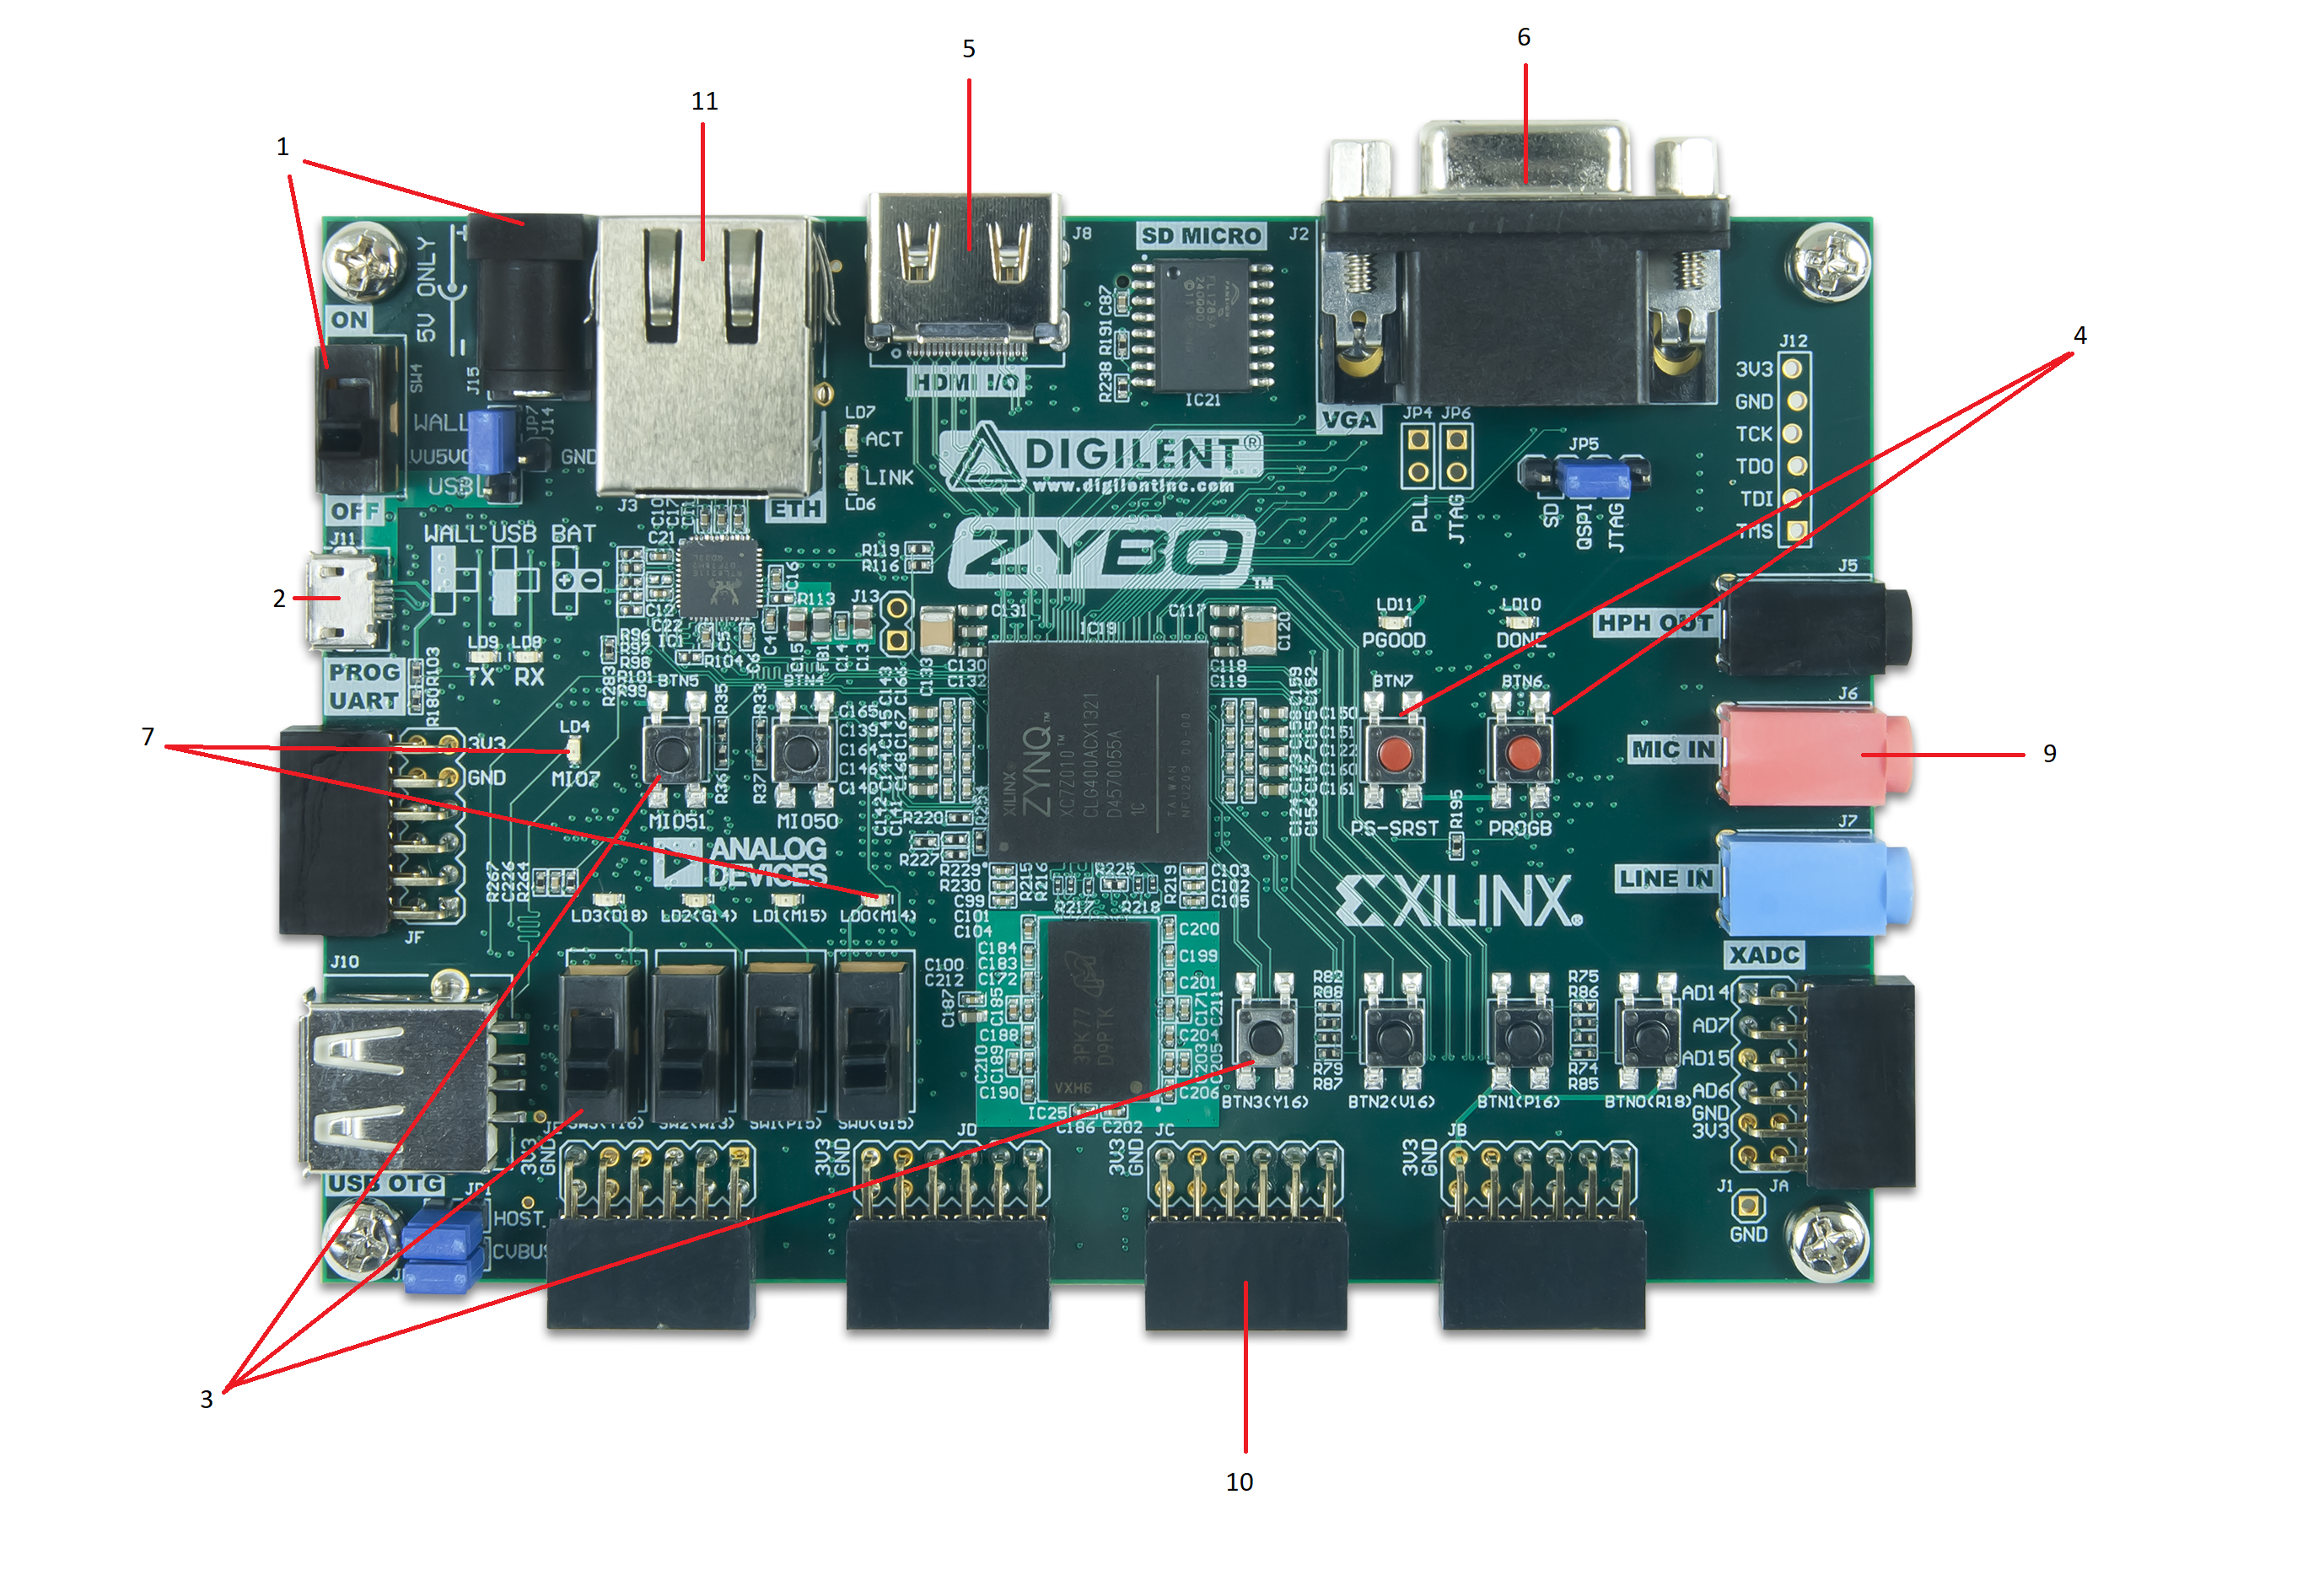
\includegraphics[width = 1\textwidth]{imagenes/zybo2.png}
    \caption{ZYBO Zynq-7000 Development Board}\label{fig:zybo}
\end{figure}

La arquitectura Zynq AP SoC está dividida en dos partes (Figura \ref{fig:zynq}), el sistema de procesamiento (\textit{PS}) y la lógica programable (\textit{PL}). 
La PL usada es parecida a la de la FPGA \textit{Xilinx 7-series Artix}, excepto porque contiene buses y puertos dedicados que hacen que esté 
acoplado fuertemente al PS. Además, la PL no tiene la misma configuración hardware como las FPGAs 7-series y tiene que ser configurada 
por el procesador o por el puerto JTAG.

\begin{figure}[H]
    \centering
    \includegraphics[width = 1\textwidth]{imagenes/zynqapsoc.png}
    \caption{Arquitectura Zynq AP SoC}\label{fig:zynq}
\end{figure}

El PS consiste en un conjunto de componentes como la \textit{APU} (Unidad de Procesamiento de Aplicaciones) que incluye dos procesadores Cortex-A9, 
\textit{AMBA} (Arquitectura de Bus de Microcontrolador Avanzada), Controlador de Memoria \textit{DDR3}, y varios controladores periféricos con 
las entradas y salidas multiplexadas a 54 pines dedicados (\textit{MIO}). Los controladores periféricos están conectados al procesador mediante 
la interconexión \textit{AMBA} y la PL está conectada de la misma manera.

Los elementos que forman la tarjeta Zybo son (Figura \ref{fig:zybo}):
\begin{enumerate}
    \item \textbf{Interruptor y Conector de alimentación}
    \item \textbf{Botones e interruptores} 
    \item \textbf{Botones de reset} 
    \item \textbf{Puerto HDMI} 
    \item \textbf{Puerto VGA} 
    \item \textbf{LEDs} 
    \item \textbf{Conectores de audio} 
    \item \textbf{Conectores Pmod} 
    \item \textbf{Conector Ethernet}
\end{enumerate}

La tarjeta Zybo incluye cuatro interruptores, cuatro botones y cuatro LEDs individuales a la PL. Además hay 2 botones y un LED conectados 
directamente al PS vía través de pines MIO. Adicionalmente hay un LED de encendido de la tarjeta, otros dos para el estado del puerto USB 
y un último LED para el estado de la programación de la FPGA.

Uno de los \textbf{botones de reset} reestablece la PL, que permanecerá sin configurar hasta ser reprogramado de nuevo. El otro reinicia 
el dispositivo sin afectar al entorno de depuración. 

Nos encontramos con tres \textbf{Conectores de audio}, dos entradas para micrófono y línea estéreo y una salida para auriculares.

El \textbf{Puerto VGA} (\textit{Video Graphics Array}) es una interfaz que recibe señal a través de un conector VGA. Éste se suele usar 
para conectar dispositivos. Está compuesto de 15 pines y cada uno tiene su propia función, entre las cuales está la de transferir los 
colores rojo, azul y verde, la sincronización horizontal y la sincronización vertical. 

El \textbf{Puerto HDMI} es un conector de entrada y salida con el que se puede transmitir vídeo compatible con HDMI o DVI. 

Los \textbf{Conectores Pmod} (\textit{Módulos Periféricos}) son unos conectores con estándares de módulos periféricos, para ampliar la capacidad de la 
lógica programable. Se comunican mediante 6,8 ó 12 pines para transportar señales de control digital. En nuestro caso, son 12 pines (2x6). 
Hay 6 conectores Pmod con distinto comportamiento en esta tarjeta y cada uno pertenece a una de las cuatro categorías, ``standard'', ``MIO connected'', 
``XADC'' y ``high-speed''.


\subsection{Vivado}

Zybo es compatible con \textit{Vivado Design Suite} de Xilinx así como con el conjunto de herramientas ISE/EDK.
Estas herramientas combinan el diseño lógico FPGA con el desarrollo software de ARM. Se pueden utilizar para diseñar sistemas 
de cualquier complejidad, desde un sistema operativo completo hasta un programa simple que controla algunos LEDs.

\textbf{Vivado Design Suite} es un entorno de diseño integrado (\textbf{IDE}) de Xilinx para la síntesis y análisis de diseños HDL. Vivado incluye 
su propio simulador lógico y además está la posibilidad de usar otros simuladores como \textit{ModelSim}, \textit{Mentor Questa}, 
\textit{Candence IES} o \textit{Synopsys VCS}. Además incluye síntesis a alto nivel con una herramienta que convierte código C a lógica
 programable.

Está formado por 4 componentes:
\begin{itemize}
    \item \textbf{Vivado High-Level Synthesis} - Permite usar programas en \(C\), \(C++\) y \(SystemC\) en dispositivos Xilinx  sin necesidad 
    de crear un RTL manualmente. Aumenta la productividad del desarrollador y admite clases, plantillas, funciones y sobrecarga de operadores.
    \item \textbf{Vivado Simulator} - Es un simulador controlado por eventos de lenguaje de descripción hardware (\textbf{HLD}) que admite 
    simulación de comportamiento y tiempos. Además admite scripts TCL (\textit{Tool Command Language}) en lenguaje mixto, es decir, admite
     lenguajes como \textit{Verilog}, \textit{SystemVerilog} y \textit{VHDL}.
    \item \textbf{Vivavo IP Integrator} - Permite integrar y  configurar IP (``\textit{Intellectual Property}") desde la biblioteca propia de Xilinx.
    \item \textbf{Vivado TCL Store} - Es un sistema de comandos para desarrollar complementos para Vivado además de agregar y modificar las 
    capacidades de Vivado. Todas las funciones de Vivado se pueden controlar con los scripts TCL.
\end{itemize}

En concreto, la versión que se ha utilizado es con Vivado 2016.2. Para trabajar con él, se puede hacer tanto trabajando con la TCL o 
directamente con la GUI de Vivado IDE \cite{vivadoIDE}. 
\begin{figure}[H]
    \centering
    \includegraphics[width = 1\textwidth]{imagenes/Vivado1.png}
    \caption{Vivado IDE}\label{vivadoGUI}
\end{figure}

La sección \textbf{Quick Start} nos proporciona fácil acceso a la creación de un nuevo proyecto, abrir proyectos existentes o abrir proyectos 
de ejemplo ofrecidos por Xilinx. Además, en la sección \textbf{Recent Projects} se pueden abrir proyectos usados recientemente.

En la sección \textbf{Tasks} encontramos el acceso a \textbf{Manage IP} que nos permite ver el catálogo de IP, personalizar IP y generar 
productos de salida.  \textbf{Open Hardware Manager} nos permite conectar la tarjeta y descargar un programa en el dispositivo FPGA. 
\textbf{Xilinx TCL Store} es un repositorio de código TCL. Da acceso a múltiples scripts para resolver problemas y mejorar la productividad.

La última sección es \textbf{Information Centre} donde se encuentra el acceso directo a la documentación, tutoriales y videos sobre lo que se 
puede hacer con esta herramienta.

Los componentes principales del entorno principal de Vivado (ver Figura \ref{vivado2} son:
\begin{enumerate}
    \item \textit{Menu Bar}
    \item \textit{Main Toolbar}
    \item \textit{Flow Navigator}
    \item \textit{Layout Selector}
    \item \textit{Data Windows Area}
    \item \textit{Workspace} 
    \item \textit{Menu Command Search Field} 
    \item \textit{Project Status Bar} 
    \item \textit{Results Windows Area}
\end{enumerate}

\begin{figure}[H]
    \centering
    \includegraphics[width = 1\textwidth]{imagenes/vivado2.png}
    \caption{Entorno Principal Vivado IDE}\label{vivado2}
\end{figure}

%\textit{Menu Bar} nos da acceso a los comandos de Vivado IDE. Normalmente, cuando se inicia un proyecto, no todos los comandos están 
%disponibles, sino que algunos se muestran cuando el diseño está activo.

%\textit{Menu Command Search Field} se encuentra a la derecha del anterior y permite localizar y ejecutar un comando de manera más rápida. La 
%lista de comandos que aparecen en la búsqueda están basados en el contexto del proyecto del diseño actual.

%\textit{Main Toolbar} nos da acceso a los comandos más usados en Vivado IDE. Si se pone el cursor en alguno de estos comandos, Vivado 
%ofrece más información acerca del mismo.

\textit{Flow Navigator} (Figura \ref{flownavigator}) permite acceder a comandos y herramientas que van desde abrir diseños a crear un archivo bitstream. Las 
diferentes secciones permiten hacer lo siguiente:
\begin{itemize}
    \item \textit{\textbf{Project Manager}}: Cambio de ajustes generales, añadir o crear archivos o abrir el Catálogo de IPs
    \item \textit{\textbf{IP Integrator}}: Crear, abrir o generar un bloque de diseño. 
    \item \textit{\textbf{Simulation}}: Cambio de ajustes de simulación o simular un diseño activo.
    \item \textit{\textbf{RTL Analysis}}: Abrir un diseño elaborado o generar un diseño de diagrama de circuitos RTL.
    \item \textit{\textbf{Synthesis}}: Cambio de ajustes de síntesis, sintetizar un diseño activo o abrir el diseño sintetizado.
    \item \textit{\textbf{Implementation}}: Cambio de ajuste de implementación, implementar un disñeo activo o abrir el diseño implementado.
    \item \textit{\textbf{Program and Debug}}: Cambio de ajustes del bitstream, generar un archivo bitstream o abrir una ventana para 
    conectar la tarjeta FPGA y programarla.
\end{itemize}

\begin{figure}[H]
    \centering
    \includegraphics[width = 0.3\textwidth]{imagenes/flownavigator.png}
    \caption{\textit{Flow Navigator}}\label{flownavigator}
\end{figure}

\textit{Layout Selector} proporciona el diseño de ventanas predefinidas para facilitar el proceso de diseño. Entre las opciones tenemos:
\begin{itemize}
    \item \textit{\textbf{Default Layout}}: Muestra el diseño con el mínimo número de ventanas, con un resumen global del diseño (Figura \ref{default}).
    \item \textit{\textbf{I/O Planning}}: Definición de restricciones de ubicación I/O y colocación de puertos (Figura \ref{io}).
    \item \textit{\textbf{Clock Planning}}: Planificación y colocación de los recursos del reloj del diseño (Figura \ref{clock}).
    \item \textit{\textbf{Floorplanning}}: Gestionar particiones y tareas jerárquicas (Figura \ref{fp}).
    \item \textit{\textbf{Timing Analysis}}: Ejecutar informes de tiempo y analizarlo (Figura \ref{ta}).
\end{itemize} 

\begin{figure}[H]
    \centering
    \includegraphics[width = 0.7\textwidth]{imagenes/default.png}
    \caption{\textit{Default Layout}}\label{default}
\end{figure}

\begin{figure}[H]
    \centering
    \includegraphics[width = 0.7\textwidth]{imagenes/io.png}
    \caption{\textit{I/O Planning}}\label{io}
\end{figure}

\begin{figure}[H]
    \centering
    \includegraphics[width = 0.7\textwidth]{imagenes/clock.png}
    \caption{\textit{Clock Planning}}\label{clock}
\end{figure}

\begin{figure}[H]
    \centering
    \includegraphics[width = 0.7\textwidth]{imagenes/fp.png}
    \caption{\textit{Floorplanning}}\label{fp}
\end{figure}

\begin{figure}[H]
    \centering
    \includegraphics[width = 1\textwidth]{imagenes/ta.png}
    \caption{\textit{Timing Analysis}}\label{ta}
\end{figure}

\textit{Project Status Bar} da información sobre el estado actual del diseño activo. \textit{Data Windows Area} muestra información 
sobre los archivos que forman el diseño. \textit{Workspace} muestra ventanas como el editor de textos o el diseño del diagrama de 
circuitos, entre otros. Y \textit{Results Windows Area} presenta los resultados de los comandos ejecutados. Además se muestran 
distintas ventanas, como \textit{Tcl Console}, \textit{Messages}, \textit{Log}, \textit{Reports} y \textit{Design Runs}.

\section{Metodología}

En esta sección se trata de estudiar y describir cómo se realiza con Vivado la metodología propia de flujo de diseño con FPGAs a partir de
descripciones RT en VHDL.

Las etapas del flujo de diseño en FPGAs son \cite{smith2010fpgas}:

\begin{enumerate}
    \item \textbf{Diseño}
    \item \textbf{Síntesis}
    \item \textbf{Simulación}
    \item \textbf{Implementación}
    \item \textbf{Generación Bitstream}
\end{enumerate}

\subsection{Diseño}

Vivado soporta múltiples lenguajes de descripción hardware, entre ellos VHDL y Verilog, e incluso se pueden usar ficheros con ambos lenguajes. 
El siguiente diagrama (Ver Figura \ref{Dflow}) muestra un flujo de diseño típico con las herramientas de Xilinx.

\begin{figure}[H]
    \centering
    \includegraphics[width = 0.5\textwidth]{imagenes/flujo.png}
    \caption{\textit{Typical Xilinx FPGA Development Flow}}\label{Dflow}
\end{figure}

Para comenzar con todo este proceso, primero tenemos que crear un proyecto. En Vivado los pasos a seguir son \textit{Create New Project} 
$\rightarrow$ \textit{Project Name} $\rightarrow$ \textit{Proyect Type} $\rightarrow$ \textit{Default Part}. En la parte \textit{Proyect Type} 
se pueden agregar ficheros en VHDL y en la parte \textit{Default Part} se establece la tarjeta que se va a configurar, en nuestro caso, 
la tarjeta ZYBO. 

Además de agregar ficheros, Xilinx nos da la opción de crear el diseño sin tener que escribir o agregar ficheros con un generador automático 
(\textit{Core Generator}), del que se hablará más adelante.

Cuando se crea el proyecto, podemos agregar nuevos ficheros con la opción \textit{Flow Navigator} $\rightarrow$ \textit{Project Manager} 
$\rightarrow$ \textit{Add Sources}.

En caso de querer cambiar la tarjeta que hemos elegido anteriormente sólo tenemos que cambiarlo en la sección \textit{Proyect Manager} en el 
apartado \textit{Proyect Settings}, además del lenguaje usado, la librería y el nombre del módulo principal.

\subsection{Simulación}

Cuando ya tenemos el diseño, hay que comprobar wl correcto funcionamiento del circuito. Para ello, se usa la simulación, que puede realizarse después del 
diseño, de la síntesis o de la implementación. A veces, la simulación se olvida por lo que lleva a largos tiempos de verificación y depuración. 

La simulación requiere de un diseño, ya sea un código o una netlist o una implementación completa y la definición de estímulos correspondientes a las 
señales de entrada del circuito como un banco de pruebas (``\textit{Testbench}''). Un banco de pruebas es uno o más módulos que conectan el diseño, 
la Unidad Bajo Prueba(\textit{UUT}), con estímulos generados desde un archivo para controlar las de la UUT y poder estudiar sus salidas.

Vivado integra su propia herramienta de simulación, aunque existe la posibilidad de usar otras herramientas como \textit{ModelSim}, \textit{Questa Advance}, 
\textit{Incisive Enterprise Simulator} o \textit{Verilog Compiler Simulator}.

Estas herramientas además de hacer uso de un banco de pruebas nos da la posibilidad de manejar las señales de entrada que queremos aplicar 
al diseño y se muestra de manera gráfica las salidas proporcionadas por el circuito además de unas listas con los componentes de los que se 
quiera conocer el estado.

\renewcommand{\theenumi}{\Alph{enumi}}
%\renewcommand{\theenumi}{\arabic{enumi}}

Hay cuatro ubicaciones principales donde ejecutar la simulación (Ver Figura \ref{Dflow}):
\begin{enumerate}
    \item ``\textbf{Behavioral Simulation}'' - Se realiza antes de la síntesis.
    \item ``\textbf{Netlist Simulation}'' - Se realiza después de la síntesis.
    \item ``\textbf{Post-Map simulation}''- Simulación posterior al mapeado tecnológico.
    \item ``\textbf{Post-Implementation}'' - Simulación después de la implementación.
\end{enumerate}

\textbf{A.} Esta simulación se conoce como simulación de comportamiento o funcional. Como sólo se dispone 
del código y no se sabe cómo se va a implementar el diseño, esta simulación se usa para comprobar la 
función de los módulos realizados. Esta es la simulación que se va a usar durante la realización de los 
casos prácticos posteriores. Para ejecutar esta simulación Vivado nos ofrece la opción \textit{Flow Navigator} 
$\rightarrow$ \textit{Simulation} $\rightarrow$ \textit{Run Simulation} $rightarrow$ \textit{Run 
Behavioral Simulation}.

\textbf{B.} Esta simulación ejecuta la versión del diseño con la lista de conexiones que contiene 
información sobre los recursos pero no la ubicación final, por lo que no hay información de enrutamiento. 
La simulación post-síntesis variará en el tiempo de la pre-síntesis, pero el comportamiento debe ser el 
mismo. Por lo tanto, esta simulación nos sirve para verificar la generación de las conexiones. En Vivado 
podemos acceder con \textit{Flow Navigator} $\rightarrow$ \textit{Simulation} $\rightarrow$ \textit{Run 
Simulation} $rightarrow$ \textit{Run Post-Synthesis Simulation}.

\textbf{C.} La simulación posterior al mapeado tecnológico no se suele ejecutar y por lo tanto no tenemos opción en Vivado. 
Pero en ella se conocen conocimientos sobre estrategia de implementación y a veces la ubicación física para 
generar una simulación de tiempo más detallada.

\textbf{D.} Esta simulación es la más precisa ya que se conocen todos los retardos. Si el diseño simula 
correctamente, pasa el análisis de tiempo y el banco de pruebas es válido, entonces la FPGA debería funcionar 
correctamente. Es la simulación que requiere más tiempo y recursos tanto en tiempo de procesador como en la redacción 
de un banco de pruebas de calidad. En algunas fases de determinados proyectos esta simulación no se realiza, sino que se 
realizan pruebas directamente configurando la FPGA de la tarjeta. Para usar esta simulación Vivado tiene 
la siguiente opción \textit{Flow Navigator} $\rightarrow$ \textit{Simulation} $\rightarrow$ \textit{Run 
Simulation} $rightarrow$ \textit{Run Post-Implementation Simulation}.

\subsection{Síntesis}

El proceso de síntesis consiste en convertir los archivos VHDL en una netlist, que es una lista de elementos 
lógicos y otra de conexiones que describe cómo se conectan los elementos. Una netlist puede ser independiente 
de la plataforma. 

Todos los errores generados por las herramientas de síntesis se deben resolver antes de pasar al siguiente 
paso, y además generan bastante advertencias que no pueden ignorarse porque pueden ocasionar errores más adelante.

Muchos entornos de desarrollo proporcionan herramientas adicionales, como visores de netlist. Vivado lo integra y
 tiene un apartado especial, \textit{Synthesis}, dentro de \textit{Flow Navigator}. Además de 
configurar los ajustes de síntesis y hacer ejecutarla, encontramos una serie de opciones que se pueden usar 
después de haberla ejecutado. Entre ellas encontramos \textit{Schematic} que nos muestra el esquemático de nuestro 
diseño, \textit{Constraints Wizard} que es un asistente para crear restricciones de tiempo con la metodología 
de diseño de Xilinx además de analizar las restricciones de tiempo que faltan en el diseño y hacer recomendaciones. 
\textit{Edit Timing Constraints} nos ayuda a modificar las restricciones creadas anteriormente. Y por último 
hay una serie de informes que nos indican el estado del diseño, entre ellos, está el informe resumido de tiempos, 
el informe de interacción de relojes, el informe sobre la utilización de elementos o el informe sobre la estimación 
de energía de la netlist de la síntesis. 

Los factores más importantes a la hora de convertir el código a un circiuto equivalente son la descripción 
del circuito, los recursos disponibles y las directivas de síntesis elegidas. A la hora de la descripción 
no sólo se establece cómo va a funcionar el circuito sino que también se decribe cómo se hace. Los recursos 
afecta a la interpretación e implementación de las funciones en recursos lógicos. Y las directivas son los 
parámetros configurables que se tienen en cuenta cuando se implementan las funciones.

El flujo del proceso de síntesis para por la comprobación del diseño, la optimización y el mapeado de la tecnología.

La netlist creada aquí pueden tener distintos formatos, como EDIF / EDF / SEDIF / EDN. Vivado usa el formato 
EDIF (``\textit{Electronic Design Interchange Format}'').

\subsection{Implementación}
\renewcommand{\theenumi}{\arabic{enumi}}

También conocida como ``\textit{Place and Route}'' consiste en convertir una o más netlist en un patrón específico 
de FPGA, es decir, transforma la netlist obtenida durante el proceso de síntesis y la mapea en la arquitectura 
de la FPGA. Este proceso se divide en los siguientes subpasos (Figura \ref{Dflow}):

\begin{enumerate}
    \item ``\textbf{Translation}''
    \item ``\textbf{Mapping}''
    \item ``\textbf{Place-and-Route}''
\end{enumerate}

\textbf{1. Translate}. El trabajo del traductor es recopilar las netlists en una sola gran netlist y 
verificar que se cumplan las restricciones. Si algún módulo no ha sido detectado en el proceso de síntesis, 
en esta etapa se marcará.

\textbf{2. Mapping}. Se encarga de comparar los recursos especificados en la netlist creada en el anterior paso 
con los recursos de la FPGA objetivo. Si no están especificados todos los recursos o hay alguno que es 
incorrecto, se mostrará un error y se detiene la implementación.

\textbf{3. Place and Route}. Es un proceso iterativo que intenta colocar (``\textit{place}'') los recursos, luego 
enruta (``\textit{route}'') las señales entre los recursos cumpliendo las limitaciones de tiempo. Esta etapa 
usa el \textbf{UCF} (``\textit{User Constraints File}'') que especifica el tiempo máximo que puede durar 
la transmisión de una señal de un recurso a otro.

Vivado tiene integrado las opciones para la realización de este proceso. En concreto, hay un apartado llamado 
\textit{Implementation} dentro de \textit{Flow Navigator}. En esta parte encontramos ajustes de implementación, 
la ejecución de la misma y una serie de opciones que se habilitan cuando se realiza todo este proceso sin errores. 
Estas opciones son las mismas que las explicadas anteriormente en el apartado de \textbf{Síntesis}. 

Cuando se quiere realizar la ejecución de la implementación, si no se ha realizado previamente la síntesis,
Vivado te muestra una advertencia de que no se ha realizado antes y después hace la ejecución de la síntesis 
y posteriormente la de la implementación como queríamos.

Una cosa importante a tener en cuenta es que si a la hora de realizar esta compilación, los pines que vayamos a 
usar no han sido asignados, nos saldrá con errores y no podremos continuar. Para que no nos suceda esto, después 
de la síntesis se pueden asignar los pines en el \textit{Layout Selector} cambiando \textit{Default Layout} por 
\textit{I/O Planning} (Ver figura \ref{io}). Otra manera sería \textit{Window} $\rightarrow$ \textit{I/O Ports}, 
pero sólo se vería la ventana donde se asignan los pines manualmente y no gráficamente como de la otra manera.

\subsection{Generación Bitstream}

El último paso es convertir el diseño que se ha generado en los pasos anteriores a un formato a un formato que 
permita configurar la FPGA asignando el valor apropiado a las celdas SRAM de configuración del dispositivo. 
El fichero bitstream puede ser generado para cargarlo directamente en la FPGA a través de 
la conexión USB o en un a memoria no volátil como una \textit{PROM} (``\textit{Programmable Read-Only Memory}'').

En Vivado hay un apartado dentro de \textit{Flow Navigator}, llamado \textit{Program and Debug} donde se puede 
generar este fichero e incluso realizar ajustes sobre el bitstream generado. Por último está \textit{Open Hardware Manager} 
que tiene tres opciones, de las cuales dos están deshabilitadas hasta que se usa la única habilitada. Esta es 
\textit{Open Target} que nos permite conectar la tarjeta al ordenador. Para saber que no ha habido ningún error 
en la conexión, en Vivado nos debería de mostrar el nombre de la tarjeta (Ver Figura \ref{hardware})

\begin{figure}[H]
    \centering
    \includegraphics[width = 0.5\textwidth]{imagenes/hardware.png}
    \caption{\textit{Hardware Manager}}\label{hardware}
\end{figure}

Una vez hecho esto se habilita la opción \textit{Program Device} que se encarga de descargar el fichero a la 
FPGA. Y si todo está correcto se habilitará también la última opción para añadir alguna configuración a 
la memoria \textit{Add Configuration Memory Device}.

\section{Desarrollo de módulos hardware específicos}

En esta sección se van describir módulos de especial interés en la plataforma para la realización de prácticas, en concreto un
procesador específico, un módulo de memoria RAM de un sólo puerto con entradas registradas, un módulo de interfaz para sincronización 
VGA y un módulo de generación de reloj.

Vivado ofrece un catálogo IP (``\textit{Intellectual Property}'') que permite agregar módulos IP a los 
diseños. Este catálogo contiene los módulos de Xilinx, pero se puede ampliar añadiendo módulos de ``System 
Generator'' para diseños DSP (\textbf{MATLAB} \textbackslash{} \textbf{Simulink}), diseños de Vivado HLS (algoritmos 
$C / C++$), IP de terceros o diseños empaquetados como IP usando alguna herramienta de empaquetado de IP Vivado \cite{ip}.

Lós métodos disponibles para trabajar con IP en un diseño son:

\begin{itemize}
    \item Utilizar el ``\textit{Manage IP}'' para personalizar IP y generar salidas, incluyendo el \textbf{DCP} 
    (Control de Diseño Sintetizado) para guardar la configuración para su uso en otras versiones.
    \item Utilizar IP en los modos \textit{Proyecto} o \textit{No Proyecto} referenciando el archivo \textbf{XCI} 
    (``\textit{Xilinx core instance}'') creado, que es un método recomendado para trabajar con proyectos 
    grandes en los que participan varias personas.
    \item Acceder al catálogo IP desde un proyecto para personalizar y agregar un módulo IP al diseño, almacenar 
    los archivos IP localmente en el proyecto o fuera del mismo.
\end{itemize}

En este TFG se trabaja con la tercera opción. Accediendo al catálogo IP desde \textit{Flow Navigator} $\rightarrow$ 
\textit{Project Manager} y vemos toda la selección de IP disponibles (Ver Figura \ref{catalogo})

\begin{figure}[H]
    \centering
    \includegraphics[width = 1\textwidth]{imagenes/catalogoip.png}
    \caption{\textit{IP Catalog}}\label{catalogo}
\end{figure}

El procesador es una adaptación del procesador propuesto en el Capítulo 9 de \cite{hamblen2007rapid}, el 
módulo de sincronización está basado en el propuesto en el Capítulo 10 del mismo libro. Los otros módulos 
se obtienen a partir del catálogo de componentes IP de Vivado.

\subsection{Procesador específico}

\subsection{Memoria RAM de un sólo puerto con entradas registradas}

Para poder tener un bloque de memoria ya definido tenemos que seleccionar \textit{IP Catalog} en el \textit{Proyect 
Manager}. Con esto, nos saldrá una lista de módulos IP disponibles. Lo que buscamos se encuentra en 
\textit{Memories and Storage Elements} $\rightarrow$ \textit{RAMs and ROMs and BRAM} y su nombre es 
\textbf{Block Memory Generator}. Al seleccionarlo tendremos un asistente de configuración que nos ayudará 
a poder definir la memoria como queramos (Ver Figura \ref{memoria}).

\begin{figure}[H]
    \centering
    \includegraphics[width = 1\textwidth]{imagenes/blockmemory.PNG}
    \caption{\textit{Block Memory Generator}}\label{memoria}
\end{figure}

Este asistente construye una memoria que utiliza memorias optimizadas para área y rendimiento usando recursos 
de bloques RAM integrados en FPGAs de Xilinx \cite{memoria}.

Este módulo tiene dos puertos independientes que acceden a un espacio de memoria compartida, teniendo ambos 
interfaz de lectura y escritura. En algunas arquitecturas FPGA de la serie \textit{UltraScale}, cada una de 
las cuatro interfaces se pueden configurar con un ancho de datos diferente. En caso de no usar las cuatro, se puede 
seleccionar una configuración de memoria simplificada, por ejemplo, una memoria con un único puerto o 
una memoria con doble puerto, para reducir la utilización de recursos de la FPGA.

La interfaz utilizada puede ser ``\textit{Native}'' o ``\textit{AXI}''. En este domucumento nos vamos a 
centrar en la primera opción. 

Se pueden generar cinco tipos de memorias, \textit{Single-port RAM}, \textit{Simple Dual-port RAM}, 
\textit{True Dual-port RAM}, \textit{Single-port ROM} y \textit{Dual-port ROM}. Para las memorias con 
dos puertos, cada uno de ellos es independiente en el modo de funcionamiento, la frecuencia 
de reloj, registros de salida opcionales y pines se pueden seleccionar por puerto.

Otra parte importante de este módulo es la selección del algoritmo usado para unir las primitivas del bloque 
RAM:

\begin{itemize}
    \item \textbf{Algoritmo de área mínima}: La memoria se genera usando el mínimo número de primitivas 
    de bloque RAM. Se usan tanto datos como bits de paridad.
    \item \textbf{Algoritmo de baja potencia}: La memoria se genera de manera que se habilita el mínimo 
    número de primitivas de bloque RAM durante la operación de lectura o escritura.
    \item \textbf{Algoritmo de primitiva fija}: La memoria se genera usando sólo un tipo de primitiva de 
    bloque RAM.
\end{itemize}

Se pueden generar bloques de memoria con estructuras de 1 a 4608 bits de ancho y al menos dos 
ubicaciones de profundidad. La profundidad máxima de la memoria está limitada sólo por el número de 
primitivas de bloque RAM en el dispositivo de destino. 

Además admite varios modos de funcionamiento de primitivas de bloque RAM como ``\textit{WRITE FIRST}'', 
``\textit{READ FIRST}'' y ``\textit{NO CHANGE}'' y a cada puerto se le puede asignar un propio modo de 
funcionamiento.

Está la opción de habilitar escritura que proporciona soportede escritura de bytes para anchos de memoria que 
son múltiplos de ocho (sin paridad) o nueve (con paridad).

También se proporcionan dos etapas opcionales de registro de salida para aumentar el rendimiento de la memoria. 
Estos registros se pueden elegir por separado para los dos puertos. 

Hay dos pines principales que son opcionales, el pin ``\textit{enable}'' que hace que se permita controlar 
el funcionamiento de la memoria, y si está desativado, no se realizan operaciones de lectura, escritura o 
reseteo en el puerto correspondiente. Si no se usa este pin, el puerto por defecto está habilitado. Y el 
pin ``\textit{reset}'' que inicializan la salida de lectura de cada puerto a un valor programable.

La memoria tiene una opción para incializarla opcionalmente, usando un archivo \textbf{COE} o usando una 
opción de datos predeterminada. Un archivo \textbf{COE} puede definir el contenido inicial de cada ubicación 
de memoria individual, mientras que la opción de datos predeterminada define el contenido inicial de todas 
las ubicaciones.

\subsection{Módulo de generación de reloj}

(Tendrías que describir el componente IP configurable y cómo se particulariza para generar la
señal de frecuencia deseada; similar a lo que se has hecho para el módulo de memoria)

\subsection{Controlador VGA}
(configurable?)



\section{Casos prácticos}

Para probar los módulos de la sección anterior, se realizan dos prácticas: un computador básico que conecta el procesador con el
módulo de memoria RAM y visualización y movimiento de objetos en monitor VGA.

\subsection{Computador básico}

\subsection{Visualización y movimiento de objetos en monitor VGA}

\textbf{Contador 4 bits}

Para la primera toma de contacto se ha realizado este simple ejemplo con el que se pretende conocer los elementos 
de la tarjeta \textbf{Zybo} además de conocer las diferentes fases de flujo de diseño con Vivado.

Se ha comenzado creando un proyecto en Vivado con el siguiente código en \textit{VHDL}. Para la verificación de su 
funcionalidad se hizo una simulación de comportamiento (Ver Figura \ref{contador}).

\begin{lstlisting}
    library ieee;
    use ieee.std_logic_1164.all;
    use ieee.std_logic_arith.all;
    use ieee.std_logic_unsigned.all;

    entity contador_4bits is
        Port(	Reloj		: IN	std_logic;
                Reset		: IN 	std_logic;
                Salida		: OUT	std_logic_vector(3 downto 0));
    end contador_4bits;

    architecture funcional of contador_4bits IS
    signal Contador : std_logic_vector(3 downto 0):="0000"; --valores 0 a 255;
    begin
        process (Reloj, Reset)
        begin
        if Reset='1' then Contador <= "0000";
            elsif reloj'event AND reloj = '1' then Contador <= Contador + 1;			
            end if;
        end process;
        Salida <= Contador;
    end funcional;
\end{lstlisting}

Para poder comprobar que la simulación funciona correctamente se necesita un testbench o bien 
añadir las señales manualmente durante la simulación.

\begin{figure}[H]
    \centering
    \includegraphics[width = 1\textwidth]{imagenes/contador4bits.png}
    \caption{\textit{Simulación Contador 4 Bits}}\label{contador}
\end{figure}

Si las salidas simuladas son correctas, se realiza la \textit{Synthesis}, donde podemos ver netlist resultante (Ver Figura \ref{netlist}).

\begin{figure}[H]
    \centering
    \includegraphics[width = 1\textwidth]{imagenes/netlist1.png}
    \caption{\textit{Netlist Resultante Synthesis}}\label{netlist}
\end{figure}

Si la comilación ha salido bien, ejecutamos la \textit{Implementation}, y si no tenemos ningún error añadimos las restricciones de la tarjeta 
que estamos utilizando (\textit{Add sources} $\rightarrow$ \textit{Add or create constraints}). Además hay que asignar los pines correctamente, en 
este ejemplo, sólo se necesita el reloj, el reset y los LEDs.

Cuando esté todo hecho, se crea el bitstream y si no hay ningún error se lleva a la FPGA. Debido a la frecuencia a la que trabaja la FPGA, la salida 
de los LEDs no es la del contador, sino una luz verde fija. Para arreglar esto, tenemos que añadir un divisor de frecuencias como el que se muestra 
a continuación.

\begin{lstlisting}
    library ieee;
    use ieee.std_logic_1164.all;
    use ieee.std_logic_arith.all;
    use ieee.std_logic_unsigned.all;
    --------------
    Entity Div_Frec is
        Port(	Velocidad 	: IN std_logic_vector(0 to 2);
                Reloj			: IN	std_logic;
            Salida		: OUT	std_logic);
    End Div_Frec;
    --------------
    Architecture funcional of Div_Frec IS
    Signal Contador : std_logic_vector(25 downto 0); --valores 0 a 67108863;
    signal Salida_int : std_logic;
    begin
        process (Reloj)
        begin
            if reloj'event AND Reloj = '1' then		
                Contador <= Contador + 1;
                Salida <= Salida_int;
            end if;
        end process;

        Salida_int <= 	contador(25) WHEN velocidad = "000" ELSE
                contador(24) WHEN velocidad = "001" ELSE
                contador(23) WHEN velocidad = "010" ELSE
                contador(22) WHEN velocidad = "011" ELSE
                contador(21) WHEN velocidad = "100" ELSE
                contador(20) WHEN velocidad = "101" ELSE
                contador(19) WHEN velocidad = "110" ELSE
                contador(18) WHEN velocidad = "111" ELSE '0';
    end funcional;
\end{lstlisting}

Pero no basta sólo con añadir este archivo, necesitamos otro archivo que una estos dos anteriores. 

\begin{lstlisting}
    LIBRARY IEEE;
    USE IEEE.STD_LOGIC_1164.all;
    USE  IEEE.STD_LOGIC_ARITH.all;
    USE  IEEE.STD_LOGIC_UNSIGNED.all;
    
    ENTITY Top IS
        PORT(
            btn       			: IN	STD_LOGIC_VECTOR(2 downto 0);
            clk					: IN	STD_LOGIC;
            rst   				: IN    STD_LOGIC;
            led                 : OUT	STD_LOGIC_VECTOR(0 TO 3));
    END Top;
    
    ARCHITECTURE estructural OF Top IS
    
        COMPONENT Div_Frec is 
        Port(	Velocidad 	: IN 	std_logic_vector(2 downto 0);
                Reloj	    : IN	std_logic;
                Salida		: OUT	std_logic);
        END COMPONENT;
    
        COMPONENT contador_4bits is 
        Port(	Reloj		: IN	std_logic;
                Reset		: IN	std_logic;
                Salida	    : OUT	std_logic_vector(3 downto 0));
        END COMPONENT;
            
        SIGNAL   CKcont : std_logic;
    
    BEGIN
        
    
        DivisorFrecuencia: Div_Frec PORT MAP(
                                    Velocidad => btn,
                                    Reloj =>    clk,
                                    Salida =>   CKcont);
                                    
        Contador4: contador_4bits PORT MAP(
                                    Reloj => CKcont,
                                    Reset => rst,
                                    Salida =>  led);	
    
    END estructural;
\end{lstlisting}

Ahora se vuelve a realizar lo mismo que antes y ya si se puede ver el contador reflejado en los LEDs de la tarjeta. 
Además con los interruptores se puede aumentar la frecuencia o disminuirla.

\textbf{Procesador}

La finalidad de esta parte es diseñar un procesador en VHDL, comprendiendo la descripción inicial de un procesador sencillo 
de 4 instrucciones, haciendo uso de una memoria RAM.

Para ello primero tenemos que crear la memoria RAM con interfaz tipo ``\textit{Native}'', 
memoria ``\textit{Single Port RAM}'', algoritmo de mínima área, ancho de escritura y lectura de 16 bits, profundidad de escritura 
y lectura de 256 bits, modo de operación ``\textit{Read First}'', sin registros de salida e incluyendo un archivo .coe inicial como 
el siguiente.

\begin{lstlisting}    
memory_initialization_radix = 16;

memory_initialization_vector =
0213,
0014,
0015,
0110,
0304,
0000,
0000,
0000,
0000,
0000,
0000,
0000,
0000,
0000,
0000,
0000,
0000,
0000,
0000,
0001,
0002,
0003,
0000;
\end{lstlisting}

Una vez generado el módulo IP, tenemos que simularlo para comprobar cómo funciona y si se ha configurado bien (Figura \ref{memoria}). 
Se puede observar que la salida ``douta'' muestra los primeros valores del archivo de inicialización siendo ``addra'' la dirección 
donde se encuentra cada uno de ellos.

\begin{figure}[H]
    \centering
    \includegraphics[width = 1\textwidth]{imagenes/memoria.png}
    \caption{\textit{Simulación Memoria RAM}}\label{memoria}
\end{figure}

Como ya lo tenemos creado, incluimos los ficheros donde se encuentra la descripción del procesador, el fichero principal donde 
se crean los componentes del procesador y de la memoria y además las restricciones de la tarjeta.

\begin{lstlisting}
library iee;
use iee.std_logic_1164.all;
use iee.std_logic_arith.all;
use iee.std_logic_signed.all;

entity procesador is
  port( clock : in std_logic;
		reset : in std_logic;
		AC_out : out std_logic_vector(15 downto 0);
		IR_out : out std_logic_vector(15 downto 0);
		PC_out : out std_logic_vector(7 downto 0);
		MEMq : in std_logic_vector(15 downto 0);
		MEMdata: out std_logic_vector(15 downto 0);
		MEMwe : out std_logic;
		MEMadr : out std_logic_vector(7 downto 0);
		IO_input : in std_logic_vector(7 downto 0);
		IO_output : out std_logic_vector(7 downto 0)
	  );
end procesador;

architecture Behavioral of procesador is

    TYPE STATE_TYPE IS ( reset_pc, fetch1, fetch0, decode, add2, add1, add0, load1, load0,
						 store0, store1, jump, sub0, sub1, nand0, nand1,
						 jneg, jpos, jzero, shr0, shl0, in1, out1);
	SIGNAL state: STATE_TYPE;
	SIGNAL IR, AC, RT: STD_LOGIC_VECTOR(15 DOWNTO 0 );
	SIGNAL PC : STD_LOGIC_VECTOR( 7 DOWNTO 0 );
	
	BEGIN
		
	-- Asignaciones a puertos de salida
	--	
	AC_out <= AC;
	IR_out <= IR;
	PC_out <= PC;


FSMD: PROCESS ( CLOCK, RESET, state, PC, AC, IR )

BEGIN

-- Asignaciones a REGISTROS en datapath y MAQUINA DE ESTADOS de la unidad de control

--version original
IF reset = '1' THEN
	state <= reset_pc;
	ELSIF clock'EVENT AND clock = '1' THEN
	 CASE state IS   
		WHEN reset_pc =>
			PC	<= "00000000";
			AC <= "0000000000000000";
			state <= fetch0;
		WHEN fetch0 =>		
			state <= fetch1;		
		WHEN fetch1 =>
			IR <= MEMq;
			PC <= PC + 1;
			state <= decode;	
		WHEN decode =>
			CASE IR( 15 DOWNTO 8 ) IS
				WHEN "00000000" =>
					state <= add0;
				WHEN "00000001" =>
					state <= store0;
				WHEN "00000010" =>
					state <= load0;
				WHEN "00000011" =>
					state <= jump;
				WHEN OTHERS =>
					state <= fetch0;
			END CASE;
		WHEN add0 => 
			state <= add1;
		WHEN add1 =>
			AC <= AC + MEMq;
			state <= fetch0;	
		WHEN store0 =>
			state <= store1;
		WHEN store1 =>
			state <= fetch0;			
		WHEN load0 =>
			state <= load1;	
		WHEN load1 =>
			AC <= MEMq;
			state <= fetch0;			
		WHEN jump =>
			PC <= IR( 7 DOWNTO 0 );
			state <= fetch0;			
		WHEN OTHERS =>
			state <= fetch0;	
	 END CASE;
	END IF;
	
-- Asignaciones a BUSES de entrada a MEMORIA (Direcciones, Datos y control de escritura)
 
 --version original
 CASE state IS
		WHEN fetch0 =>
			MEMadr <= PC;
			MEMwe <= '0';
			MEMdata <= (others =>'-');
		WHEN add0 | load0 =>
			MEMadr <= IR(7 downto 0);
			MEMwe <= '0';
			MEMdata <= (others =>'-');
		WHEN store0 => 
			MEMadr <= IR(7 downto 0);
			MEMwe <= '1';
			MEMdata <= AC;
		WHEN others =>
			MEMadr <= IR(7 downto 0);
			MEMwe <= '0';
			MEMdata <= (others =>'-');
	end case;
	
END PROCESS;

end Behavioral;
\end{lstlisting}

Este procesador puede ejecutar 4 instrucciones: \textbf{ADD}, \textbf{STORE}, \textbf{LOAD} Y \textbf{JUMP}. El repertorio 
inicial de instrucciones corresponde al del computador elemental presentado en el capítulo 9 de \cite{hamblen2007rapid}. Cada 
instrucción ocupa 16 bits. En la versión original, los primeros 8 bits (los más significativos) corresponden a un código de 
opración mientras que los restantes son la dirección.

\begin{tabular}{c l l}
    CODOP & Instrucción & Descripción \\
    00 & ADD address & AC $\leftarrow$ AC $+$ M(address) \\
    01 & STORE address & M(address) $\leftarrow$ AC \\
    02 & LOAD address &  AC $\leftarrow$ M(address) \\
    03 & JUMP address &  PC $\leftarrow$ adress\\
\end{tabular}

\begin{lstlisting}
library ieee;
use ieee.std_logic_1164.all;
use ieee.std_logic_arith.all;
use ieee.std_logic_unsigned.all;

entity my_scomp IS
port( reloj : in std_logic;
		reset : in std_logic;
		IR_out: out std_logic_vector(15 downto 0);
		AC_out: out std_logic_vector(15 downto 0);
		PC_out : out std_logic_vector(7 downto 0);
		IO_input : in std_logic_vector(7 downto 0);
		IO_output : out std_logic_vector(7 downto 0)
		);
end my_scomp;

architecture rtl of my_scomp is

	signal MEMq, MEMdata: std_logic_vector(15 DOWNTO 0 );
	signal MEMadr : std_logic_vector( 7 DOWNTO 0 );
	signal MEMwe : std_logic;
	signal reset_s : std_logic;

	-- Declaracion del IP core ram_256_x_16 
	--
	-- 	Memoria RAM de un puerto, 256 palabras, 16 bits por palabra, 
	-- 	Entradas de datos, direcciones y control de memoria REGISTRADAS, 
	-- 	Salida NO REGISTRADA 
	-- 	Fichero de inicializacion: datos.coe	
	
	component blk_mem_gen_0 is
	port
	(
		addra		: IN std_logic_vector (7 DOWNTO 0);
		clka		: IN std_logic  := '1';
		dina		: IN std_logic_vector (15 DOWNTO 0);
		wea 		: IN std_logic ;
		douta		: OUT std_logic_vector (15 DOWNTO 0)
	);
	end component;
	
	-- Declaracion del componente con version inicial del procesador 

	component procesador is
	port( clock : in std_logic;
		reset : in std_logic;
		AC_out : out std_logic_vector(15 downto 0);
		IR_out : out std_logic_vector(15 downto 0);
		PC_out : out std_logic_vector(7 downto 0);
		MEMq : in std_logic_vector(15 downto 0);
		MEMdata: out std_logic_vector(15 downto 0);
		MEMwe : out std_logic;
		MEMadr : out std_logic_vector(7 downto 0);
		IO_input : in std_logic_vector(7 downto 0);
		IO_output : out std_logic_vector(7 downto 0)
	);
	end component;
	
	begin
	
	-- Instancia denominada MEM del IP core ram_256_x_16
	
	MEM: blk_mem_gen_0	PORT MAP (
		addra => MEMadr,
		clka => reloj,
		dina => MEMdata,
		wea => MEMwe,
		douta => MEMq
	);

	-- Instancia denominada PROC de la version inicial del procesador
	--	
	
	PROC: procesador PORT MAP (
		clock => reloj, 
		reset => reset_s,
		AC_out => AC_out,
		IR_out => IR_out,
		PC_out => PC_out,
		MEMq => MEMq,
		MEMdata => MEMdata,
		MEMwe => MEMwe,
		MEMadr => MEMadr,
		IO_input => IO_input,
		IO_output => IO_output
	);

    estimulos: PROCESS 
    begin
    
        reset_s <= '1';
        WAIT FOR 10ns;
        reset_s <= '0';
        WAIT;
    
    end PROCESS;
	
end rtl;
\end{lstlisting}

Una vez añadidos estos ficheros, realizamos la simulación del conjunto (Figura \ref{procesador}). Se puede observar cómo se 
ejecuta la secuencia de instrucciones que hemos introducido en el fichero de inicialización. El procedimiento es el siguiente: 
Primero se lee lo que hay en la dirección 0, 0213, 02 indica que se va a ejecutar la instrucción LOAD, es decir, se va a leer el 
dato que haya en la dirección 13 y se va a asignar a la señal AC. Después, se pasa a la siguiente, 0014, 00 indica que se va 
a ejecutar la instrucción ADD, es decir, se va a coger lo que haya en la dirección 14, se le suma lo que se había cargado en AC y 
este resultado se vuelve a intriducir en AC. La siguiente instrucción es 0015, que hace lo mismo que la anterior. A continuación, 
la siguiente es 0110, 01 indica que se va a realizar un STORE, es decir, se va a cargar en la dirección 10 lo que había en AC. Por 
último, 0304, 03 indica que se va a hacer un JUMP, es decir, se va a saltar a la dirección 04.

\begin{figure}[H]
    \centering
    \includegraphics[width = 1\textwidth]{imagenes/procesador.png}
    \caption{\textit{Simulación Procesador}}\label{procesador}
\end{figure}

\textbf{Controlador VGA}

En esta práctica se pretende realizar una implementación de un juego interactivo tipo Pong, comprendiendo el modo de operación 
del módulo de interfaz VGA. Para ello disponemos de una descripción en vhdl del módulo de sincronismo VGA y un módulo que visualiza 
una bola que se mueve en vertical rebotando con los bordes superior e inferior de la pantalla. Además hay que usar un módulo IP que 
genera un reloj de 25MHz a partir del reloj que proporciona la tarjeta.

\begin{lstlisting}
    library IEEE;
    use  IEEE.STD_LOGIC_1164.all;
    use  IEEE.STD_LOGIC_ARITH.all;
    use  IEEE.STD_LOGIC_UNSIGNED.all;
    
    entity controlador_vga_640_x_480_60 IS
        PORT(	
                clock_25		: 	IN	STD_LOGIC;
                r,g,b	: 	IN	STD_LOGIC;
                vga_r			:	OUT	STD_LOGIC;
                vga_g		:	OUT	STD_LOGIC;
                vga_b		:	OUT	STD_LOGIC;
                vga_blank_N	:	OUT	STD_LOGIC;
                vga_hs			:	OUT STD_LOGIC;
                vga_vs			:	OUT STD_LOGIC;
                vga_clk			:	OUT STD_LOGIC;
                pixel_y			:	OUT STD_LOGIC_VECTOR(9 DOWNTO 0);
                pixel_x			:	OUT	STD_LOGIC_VECTOR(9 DOWNTO 0)
        );		
                
    END controlador_vga_640_x_480_60;
    
    ARCHITECTURE  rtl OF controlador_vga_640_x_480_60 IS
    
    -- Especificacione temporales VGA 640 x 480 pixels (60 Hz), 25M pixels/s
    -- Sincronizacion horizontal (en numero de pixels/linea)
      CONSTANT h_a: integer := 96; -- Retorno horizontal
      CONSTANT h_b: integer := 48; -- "Back porch" horizontal (Margen izquierdo)
      CONSTANT h_c: integer := 640; -- Area de visualizacion horizontal 
      CONSTANT h_d: integer := 16; -- "Front porch" horizontal (Margen derecho)  
      CONSTANT h_total : integer := h_a + h_b + h_c + h_d;  
       
    -- Sincronizacion Vertical (en numero de lineas/pantalla)  
      CONSTANT v_a: integer := 2; -- Retorno vertical
      CONSTANT v_b: integer := 33; -- "Back porch" vertical
      CONSTANT v_c: integer := 480; -- Area de visualizacion vertical 
      CONSTANT v_d: integer := 10; -- "Front porch" vertical 
      CONSTANT v_total : integer := v_a + v_b + v_c + v_d;  
     
        
        SIGNAL hs, vs : STD_LOGIC;
        SIGNAL video_on : STD_LOGIC;
        SIGNAL cont_hs, cont_vs :STD_LOGIC_VECTOR(9 DOWNTO 0);
    
    BEGIN
    
    -- La senial vga_clk que va al DAC coincide con el reloj de 25MHz. 
    vga_clk <= clock_25;
    
    PROCESS
    BEGIN
        WAIT UNTIL(clock_25'EVENT) AND (clock_25='1');
    
    
    -- Se generan las seniales de sinronizacion horizontal y vertical
    -- a partir de los contadores cont_hs y cont_vs
    
    -- El contador cont_hs cuenta los pixels/fila
    -- La senial de sincronizacion horizontal (hs) vale cero durante el retorno horizontal 
    
    --
        IF (cont_hs = h_total - 1) THEN
               cont_hs <= "0000000000";
        ELSE
               cont_hs <= cont_hs + 1;
        END IF;
    
    IF (cont_hs <= h_c+h_d+h_a-1) AND (cont_hs >= h_c+h_d) THEN
               hs <= '0';
        ELSE
               hs <= '1';
        END IF;
    
    -- El contador cont_vs cuenta las filas/pantalla
    -- La senial de sincronizacion vertical (vs) vale cero durante el retorno vertical
    
        IF (cont_vs = v_total - 1) AND (cont_hs >= h_total - h_a - h_d) THEN
               cont_vs <= "0000000000";
        ELSIF (cont_hs = h_total - h_a - h_d) THEN
               cont_vs <= cont_vs + 1;
        END IF;
    
        IF (cont_vs <= v_c+v_d+v_a-1) AND (cont_vs >= v_c+v_d) THEN
               vs <= '0';
        ELSE
               vs <= '1';
        END IF;
    
    
    -- Se generan seniales para informar a la salida de la coordenada de pixel a visualizar
        IF (cont_hs <= 639) THEN pixel_x <= cont_hs;	END IF;
        IF (cont_vs <= 479) THEN pixel_y <= cont_vs; end if; 
        
        -- La senial video_on esta en alta cuando se transmite informacion de video
      -- (para valores de cont_vs entre 0 y 479, y valores de cont_hs entre 0 y 639)
     
      if (cont_hs <= 639) and (cont_vs <= 479) then video_on <= '1'; else video_on <= '0'; end if;
    
    -- Se registran todas las seniales de video para eliminar retardos que puedan emborronar la imagen
            vga_r <= r AND video_on;
            vga_g <= g AND video_on;
            vga_b <= b AND video_on;
            vga_hs 	<= hs;
            vga_vs 	<= vs;
            vga_blank_n <= video_on;
    
    END PROCESS;
    
    END rtl;
\end{lstlisting}

Este código del controlador VGA genera señales de sincronización horizontal y vertical, utilizando contadores de 10 
bits. H\_count hace la cuenta horizontal mientras que V\_count hace la vertical. Ambos generan una dirección de píxeles 
en filas y columnas disponibles para otros procesos. Estas señales las usamos para determinar las coordenadas x e y de 
la ubicación de vídeo actual. La dirección de pixel se usa para generar los datos del color RGB de la imagen. 

La lógica interna de la mayoría de las placas usan un reloj de 25MHz generado por un PLL, módulo IP que se generará desde 
el catálogo IP. Los contadores se utilizan para producir señales de sincronización de vídeo. Para desactivar los 
datos RGB cuando no se muestran los píxeles, se genera la señal video\_on \cite{hamblen2007rapid}. 

Tras conocer el controlador VGA, hay que crear el módulo PLL. Para ello sólo tenemos que entrar en el catálogo IP de Vivado 
(\textit{FPGA Features and Design} $\rightarrow$ \textit{Clocking} $\rightarrow$ \textit{Cloking Wizard}) y configurándolo 
de manera que se seleccione la opción PLL y en la salida del reloj poner la frecuencia deseada, en este caso, 25MHz.

\textit{Clocking Wizard} crea un circuito de reloj para una frecuencia, fase y ciclo de trabajo del reloj de salida 
requeridos mediante un administrador de reloj de modo mixto (\textbf{MMCM}) o un bucle de bloqueo de fase (\textbf{PLL}). 
También ayuda a verificar la frecuencia de reloj generada por la salida en la simulación \cite{pll}.

Por último se agrega la descripción de la bola, en la que además de la bola, se especifican las palas y una red para la 
finalización del juego de un modo más sencillo.

\begin{lstlisting}
    LIBRARY IEEE;
    USE IEEE.STD_LOGIC_1164.all;
    USE IEEE.STD_LOGIC_ARITH.all;
    USE IEEE.STD_LOGIC_UNSIGNED.all;
    LIBRARY lpm;
    USE lpm.lpm_components.ALL;
    
    ENTITY bola IS
        PORT(
            Red,Green,Blue : OUT std_logic;
            vs : IN std_logic;
            pixel_Y, pixel_X : IN std_logic_vector(9 downto 0);
            up1, down1, up2, down2 : IN std_logic
            );
    END bola;
    
    architecture funcional of bola is
       -- Seniales para el tamanio de la bola y su desplazamiento
        SIGNAL Bola_on : STD_LOGIC;	-- "Dibujar" bola
        SIGNAL Desplaza_Bola_Y: STD_LOGIC_VECTOR(9 DOWNTO 0);	-- Desplazamiento en pixeles de la bola en y
        SIGNAL Desplaza_Bola_X: STD_LOGIC_VECTOR(9 DOWNTO 0);	-- Desplazamiento en pixeles de la bola en x
        SIGNAL Bola_Y  : STD_LOGIC_VECTOR(9 DOWNTO 0);	-- "Eje" y de la bola
        SIGNAL Bola_X	: STD_LOGIC_VECTOR(9 DOWNTO 0);	-- "Eje" x de la bola
        
        -- Seniales para el tamanio de la pala izquierda y su desplazamiento vertical	
        SIGNAL Pala_izq_on : STD_LOGIC;	-- "Dibujar" pala izquierda
        SIGNAL Desplaza_Pala_izq_Y: STD_LOGIC_VECTOR(9 DOWNTO 0);	-- Desplazamiento en pixeles de la pala izquierda en y
        SIGNAL Desplaza_Pala_izq_X: STD_LOGIC_VECTOR(9 DOWNTO 0);	-- Desplazamiento en pixeles de la pala izquierda en x
        SIGNAL Pala_izq_Y : STD_LOGIC_VECTOR(9 DOWNTO 0);	-- "Eje" y de la pala izquierda
        
        -- Seniales para el tamanio de la pala derecha y su desplazamiento vertical	
        SIGNAL Pala_der_on : STD_LOGIC;	-- "Dibujar" pala derecha
        SIGNAL Desplaza_Pala_der_Y: STD_LOGIC_VECTOR(9 DOWNTO 0);	-- Desplazamiento en pixeles de la pala derecha en y
        SIGNAL Desplaza_Pala_der_X: STD_LOGIC_VECTOR(9 DOWNTO 0);	-- Desplazamiento en pixeles de la pala derecha en x
        SIGNAL Pala_der_Y : STD_LOGIC_VECTOR(9 DOWNTO 0);	-- "Eje" y de la pala derecha
        
        -- Seniales para la red del campo
        SIGNAL Red_on : STD_LOGIC;
        SIGNAL Red_y : STD_LOGIC_VECTOR(9 DOWNTO 0);
        CONSTANT Red_x : STD_LOGIC_VECTOR(9 DOWNTO 0) := CONV_STD_LOGIC_VECTOR(320,10);
        CONSTANT Size_red_y : STD_LOGIC_VECTOR(9 DOWNTO 0):= CONV_STD_LOGIC_VECTOR(479,10);
        CONSTANT Size_red_x : STD_LOGIC_VECTOR(9 DOWNTO 0):= CONV_STD_LOGIC_VECTOR(1,10);
    
        CONSTANT Size_X : STD_LOGIC_VECTOR(9 DOWNTO 0):= CONV_STD_LOGIC_VECTOR(4,10);	-- Tamanio del objeto en el eje x
        CONSTANT Size_Y : STD_LOGIC_VECTOR(9 DOWNTO 0):= CONV_STD_LOGIC_VECTOR(40,10); -- Tamanio del objeto en el eje y
        CONSTANT Pala_izq_X : STD_LOGIC_VECTOR(9 DOWNTO 0):= CONV_STD_LOGIC_VECTOR(40,10);	-- "Eje" x de la pala derecha, constante
        CONSTANT Pala_der_X : STD_LOGIC_VECTOR(9 DOWNTO 0):= CONV_STD_LOGIC_VECTOR(600,10);	-- "Eje" x de la pala izquierda, constante
        
    BEGIN
    
    -- Pelota gris, pala izquierda roja y pala derecha azul
    Red	<= Bola_on OR Pala_der_on;
    Green	<= Bola_on OR Red_on;
    Blue	<= Bola_on OR Pala_izq_on OR Red_on;
    
    Dibujar_Bola: Process (Bola_Y, pixel_X, pixel_Y)
    BEGIN
        -- Chequear coordenadas X e Y para identificar el area de la bola
        -- Poner Bola_on a '1' para visualizar la bola
        IF (Bola_X <= pixel_X + Size_X) AND
            (Bola_X + Size_X >= pixel_X) AND
            (Bola_Y <= pixel_Y + Size_X) AND
            (Bola_Y + Size_X >= pixel_Y ) THEN
            
            Bola_on <= '1';
        ELSE
            Bola_on <= '0';
        END IF;
        
    END process Dibujar_Bola;
    
    Dibujar_Pala_Izq: Process (Pala_izq_Y, pixel_X, pixel_Y)
    BEGIN
        -- Chequear coordenadas X e Y para identificar el area de la pala
        -- Poner Pala_on a '1' para visualizar la pala
        IF (Pala_izq_X <= pixel_X + Size_X) AND
            (Pala_izq_X + Size_X >= pixel_X) AND
            (Pala_izq_Y <= pixel_Y + Size_Y) AND
            (Pala_izq_Y + Size_Y >= pixel_Y ) THEN
            
            Pala_izq_on <= '1';
        ELSE
            Pala_izq_on <= '0';
        END IF;
    END process Dibujar_Pala_Izq;
    
    Dibujar_Pala_Der: Process (Pala_der_Y, pixel_X, pixel_Y)
    BEGIN
        -- Chequear coordenadas X e Y para identificar el area de la pala
        -- Poner Pala_on a '1' para visualizar la pala
        IF (Pala_der_X <= pixel_X + Size_X) AND
            (Pala_der_X + Size_X >= pixel_X) AND
            (Pala_der_Y <= pixel_Y + Size_Y) AND
            (Pala_der_Y + Size_Y >= pixel_Y ) THEN
            
            Pala_der_on <= '1';
        ELSE
            Pala_der_on <= '0';
        END IF;
    END process Dibujar_Pala_Der;
    
    Dibujar_Red: Process(Red_Y, pixel_X, pixel_Y)
    BEGIN
        IF (Red_X <= pixel_X + Size_red_X) AND
            (Red_X + Size_red_X >= pixel_X) AND
            (Red_Y <= pixel_Y + Size_red_Y) AND
            (Red_Y + Size_red_Y >= pixel_Y ) THEN
            
            Red_on <= '1';
        ELSE
            Red_on <= '0';
        END IF;
    END Process Dibujar_Red;
    
    Mover_Bola: PROCESS (vs)
    BEGIN
        -- Actualizar la posicion de la bola en cada refresco de pantalla
        IF vs'event and vs = '1' THEN
            -- Detectar los bordes superior e inferior de la pantalla
                IF Bola_Y  >= CONV_STD_LOGIC_VECTOR(479,10) - Size_X THEN
                    Desplaza_Bola_Y <= CONV_STD_LOGIC_VECTOR(-2,10);
                ELSIF  Bola_Y <= Size_X  THEN
                    Desplaza_Bola_Y <= CONV_STD_LOGIC_VECTOR(2,10);
                END IF;
                -- Calcular la siguiente posicion de la bola
                Bola_Y 	  	<= Bola_Y + Desplaza_Bola_Y;
                
             --Detectar los bordes derecho e izquierdo de la pantalla
                IF Bola_X  >= CONV_STD_LOGIC_VECTOR(639,10) - Size_X THEN	
                    Desplaza_Bola_X <= CONV_STD_LOGIC_VECTOR(-2,10);				
                ELSIF  Bola_X <= Size_X  THEN											
                    Desplaza_Bola_X <= CONV_STD_LOGIC_VECTOR(2,10);
                END IF;
                --Calcular la siguiente posicion de la bola
                Bola_X 	  	<= Bola_X + Desplaza_Bola_X;
                
            -- Rebote por la derecha, pala izquierda
                IF (Bola_Y + Size_X + Size_Y >= Pala_izq_Y) AND
                    (Bola_Y <= Pala_izq_Y + Size_Y + Size_X) AND
                    (Bola_X <= Pala_izq_X + Size_X + Size_X) THEN
                    Desplaza_Bola_X <= CONV_STD_LOGIC_VECTOR(2,10);
                END IF;
                
                -- Rebote por la izquierda, pala derecha			
                IF (Bola_Y + Size_X + Size_Y >= Pala_der_Y) AND
                    (Bola_Y <= Pala_der_Y + Size_Y + Size_X) AND
                    (Bola_X + Size_X + Size_X >= Pala_der_X) THEN
                    Desplaza_Bola_X <= CONV_STD_LOGIC_VECTOR(-2,10);
                END IF;
                
        END IF;
    END process Mover_Bola;
    
    Mover_Pala_Izq: PROCESS (vs)
    BEGIN
        -- Actualizar la posicion de la bola en cada refresco de pantalla
        IF vs'event and vs = '1' THEN
            -- Detectar los bordes superior e inferior de la pantalla
                IF (down1 = '0') AND (Pala_izq_Y  <= CONV_STD_LOGIC_VECTOR(479,10) - Size_Y) THEN
                    Desplaza_Pala_izq_Y <= CONV_STD_LOGIC_VECTOR(2,10);
                ELSIF  (up1 = '0') AND (Pala_izq_Y >= Size_Y) THEN
                    Desplaza_Pala_izq_Y <= CONV_STD_LOGIC_VECTOR(-2,10);
                ELSE
                    Desplaza_Pala_izq_Y <= CONV_STD_LOGIC_VECTOR(0,10);
                END IF;
                -- Calcular la siguiente posicion de la bola
                Pala_izq_Y <= Pala_izq_Y + Desplaza_Pala_izq_Y;
        END IF;
    END process Mover_Pala_Izq;
    
    Mover_Pala_Der: PROCESS (vs)
    BEGIN
        -- Actualizar la posicion de la bola en cada refresco de pantalla
        IF vs'event and vs = '1' THEN			
            -- Detectar los bordes superior e inferior de la pantalla
                IF (down2 = '0') AND (Pala_der_Y  <= CONV_STD_LOGIC_VECTOR(479,10) - Size_Y) THEN
                    Desplaza_Pala_der_Y <= CONV_STD_LOGIC_VECTOR(2,10);
                ELSIF  (up2 = '0') AND (Pala_der_Y >= Size_Y) THEN
                    Desplaza_Pala_der_Y <= CONV_STD_LOGIC_VECTOR(-2,10);
                ELSE
                    Desplaza_Pala_der_Y <= CONV_STD_LOGIC_VECTOR(0,10);
                END IF;
                
                -- Calcular la siguiente posicion de la bola
                Pala_der_Y <= Pala_der_Y + Desplaza_Pala_der_Y;
        END IF;
    END process Mover_Pala_Der;
    
    Mover_Red: PROCESS (vs)
    BEGIN
        IF vs'event and vs = '1' THEN			
            Red_Y <= CONV_STD_LOGIC_VECTOR(0,10);
        END IF;
    END PROCESS Mover_Red;
    
    -- Los botones estan a la alta siempre que no esten pulsados
    
    END funcional;
\end{lstlisting}

Las señales pixel\_X y pixel\_Y se usan para determinar la fila y columna actuales, respectivamente. Bola\_x y Bola\_y 
son la dirección actual del centro de la bola. Size\_x es el tamaño de la bola cuadrada. El proceso Mover\_Bola, mueve la bola 
unos pocos píxeles en cada sincronización vertical y comprueba si hay rebotes en la pared. Bola\_on dibuja la bola en la 
pantalla y Desplaza\_Bola\_X y Desplaza\_Bola\_Y es el número de píxeles que la bola se tiene que mover tanto horizontal como 
verticalmente. Y para las palas y la red se ha realizado el mismo procedimiento. Las señales up1, up2, down1, down2 están 
conectadas a los pines que corresponden con los botones para hacer que las palas suben y bajen cuando se pulse alguno de 
ellos.

Una vez entendidos todos los ficheros, sólo tenemos que ejecutar la síntesis, la implementación, asignar los pines, generar el 
fichero bitstream y cargar el resultado en la FPGA. Después de esto podremos ver en la pantalla el sencillo juego y además hacer 
que las palas se muevan para poder probarlo.